\chapter{\label{ch3-architecture}CTA Architecture} 

\minitoc

\notes[inline,caption={}]{
	\section{Plan}
	\subsection{Topics}
	\begin{itemize}
		\item Requirements
		\item Data Levels
	\end{itemize}
	\subsection{Questions}
	\begin{itemize}
		\item ?
	\end{itemize}
}

\section{Introduction}

Due to the large scope of \gls{cta}, in both its construction and operation, a formal approach towards a system architecture was adopted \cite{Dazzi2018}. One important aspect within this architecture is the distinction between the \gls{cta} Consortium and the \gls{cta} Observatory. The \gls{cta} Consortium is a group of institutes responsible for directing the science goals of the observatory, and for developing software and hardware (including cameras), which are supplied to the observatory as in-kind contributions. The consortium consists of 200 institutes across 31 countries \cite{cta-consortium}. Conversely, the CTA Observatory pertains to the major astronomical facility that serves science data to a wide user community as an open observatory. The \gls{cta} Observatory gGmbH is the legal entity for \gls{cta} in the preparation for the implementation of the \gls{cta} Observatory, and works in close cooperation with the consortium during this process \cite{cta-observatory}.

The purpose of the \gls{cta} architecture is to maintain communication and understanding among all \gls{cta} contributors during the pre-construction phase in order to ensure a coherent development process and seamless integration of the developed units into a whole. During this chapter I will describe two aspects of the \gls{cta} architecture that are important in the context of this thesis: certain requirements that all cameras, including \gls{chec}, must meet; and the descriptions of how camera-observation data are handled in \gls{cta}, including the system flow and data level definitions.

\section{Requirements}

In order to ensure the science goals of \gls{cta} are achievable, certain standards must be upheld by all components of the observatory. This is the purpose of the \gls{cta} requirements. In order for an in-kind contribution to be accepted, it must meet the requirements defined by the observatory. These requirements are therefore the standards for which we compare the performance of \gls{chec} against, and are the primary drivers in my development of the low-level calibration and analysis. However, the full review of the camera is a much larger undertaking than can be covered in this thesis, and so I highlight only the requirements relevant to the work discussed.
It is important to note that the requirements, located on the \gls{cta} Jama website \cite{cta-jama}, are currently under-review and therefore subject to change. A copy of each requirement at the time of this writing is included alongside the discussion in this section to ensure clarity about which requirement definition is being referred to.

\begin{requirement}{\subsection{B-TEL-1010 Charge Resolution}}
	The required fractional Charge Resolution for Cherenkov signals in each Camera pixel for a specified background level of 0.125 photoelectrons/ns is given in the Figure below and Table attached. Charge measurements must be possible for 0-1000 photoelectron signals. The average charge resolution should be calculated for the reference Gamma-Ray Spectrum.
    
	\centering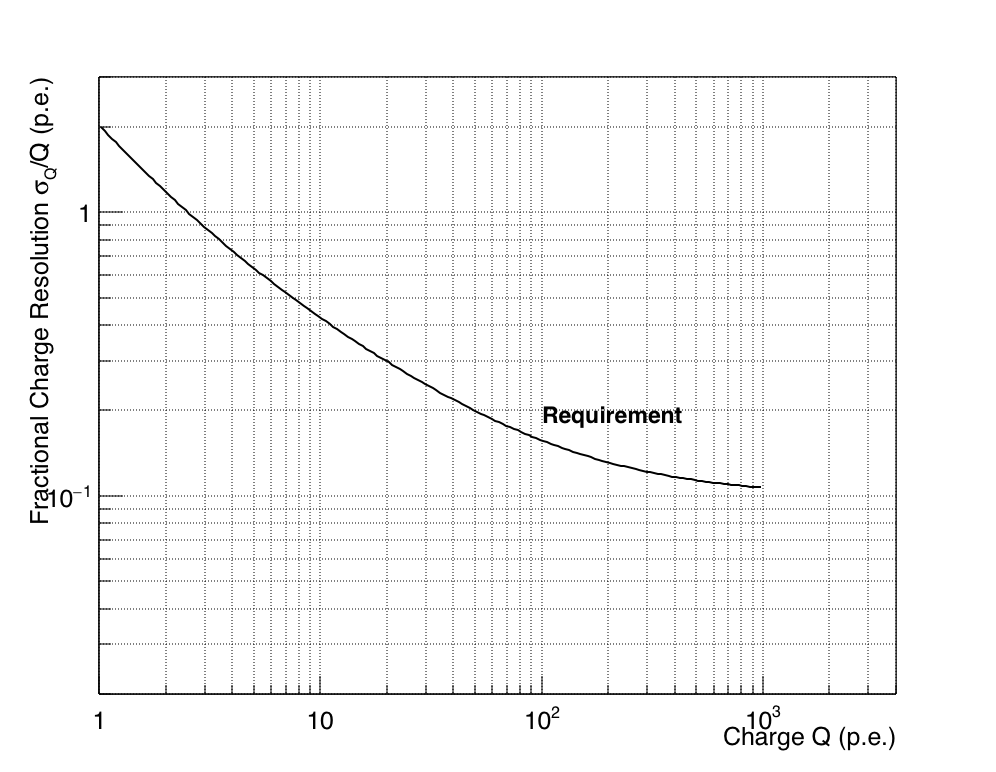
\includegraphics[width=0.8\linewidth]{figures/images/charge_res_req}
	\captionof{figure}{Fractional rms charge resolution $\sigma_Q/Q$ per pixel for different Cherenkov light signal amplitudes, expressed in units of photoelectrons (p.e.). All sources of fluctuations, including Poisson fluctuations in photoelectron number, must be included, The true pixel charge $Q$ is that measured in an ideal detector with the same photon-detection efficiency. }\label{fig:charge_res_req}
    
\begin{itemize}
\item [Notes:] It is expected that this requirement is verified with reference to:

- Monte Carlo simulation of Cherenkov light from gamma-ray initiated showers (using a verified telescope model),

- Level-C Specification on Laboratory Measured Charge Resolution,

- Monte Carlo simulation of the laboratory test set-up (as a means of telescope model verification).

Note that between 1000pe and 2000pe, some sensitivity to increasing input signal must exist. \newline
This requirement applies to post-calibration (DL1) data. \newline
Note that this requirement will likely need to be expanded to cover performance at higher NSB levels.
\end{itemize}
\end{requirement}

This requirement...

\section{Data Levels}

